% --------------------------------------------------------------------------- %
% Poster for the ECCS 2011 Conference about Elementary Dynamic Networks.      %
% --------------------------------------------------------------------------- %
% Created with Brian Amberg's LaTeX Poster Template. Please refer for the     %
% attached README.md file for the details how to compile with `pdflatex`.     %
% --------------------------------------------------------------------------- %
% $LastChangedDate:: 2011-09-11 10:57:12 +0200 (V, 11 szept. 2011)          $ %
% $LastChangedRevision:: 128                                                $ %
% $LastChangedBy:: rlegendi                                                 $ %
% $Id:: poster.tex 128 2011-09-11 08:57:12Z rlegendi                        $ %
% --------------------------------------------------------------------------- %
\documentclass[a0paper,portrait]{baposter}

\usepackage[ngerman]{babel}
\usepackage{relsize}		% For \smaller
\usepackage{url}			% For \url
\usepackage{epstopdf}	% Included EPS files automatically converted to PDF to include with pdflatex
\usepackage{tikz}
\usepackage{blindtext,multicol,fontspec}
\setmainfont{Linux Libertine O}

%%% Global Settings %%%%%%%%%%%%%%%%%%%%%%%%%%%%%%%%%%%%%%%%%%%%%%%%%%%%%%%%%%%

\graphicspath{{Bilder/}}	% Root directory of the pictures 
\tracingstats=2			% Enabled LaTeX logging with conditionals

%%% Color Definitions %%%%%%%%%%%%%%%%%%%%%%%%%%%%%%%%%%%%%%%%%%%%%%%%%%%%%%%%%

\definecolor{bordercol}{RGB}{40,40,40}
\definecolor{headercol1}{RGB}{150,200,255}
\definecolor{headercol2}{RGB}{72,61,139}
\definecolor{headerfontcol}{RGB}{0,0,0}
\definecolor{boxcolor}{RGB}{240,270,255} %%gut: 230:291:255
\definecolor{boxColorTwo}{RGB}{80,80,80}
\definecolor{bgColor1}{RGB}{235,255,250}
\definecolor{bgColor2}{RGB}{70,70,255}

%%%%%%%%%%%%%%%%%%%%%%%%%%%%%%%%%%%%%%%%%%%%%%%%%%%%%%%%%%%%%%%%%%%%%%%%%%%%%%%%
%%% Utility functions %%%%%%%%%%%%%%%%%%%%%%%%%%%%%%%%%%%%%%%%%%%%%%%%%%%%%%%%%%

%%% Save space in lists. Use this after the opening of the list %%%%%%%%%%%%%%%%
\newcommand{\compresslist}{
	\setlength{\itemsep}{1pt}
	\setlength{\parskip}{0pt}
	\setlength{\parsep}{0pt}
}

%%%%%%%%%%%%%%%%%%%%%%%%%%%%%%%%%%%%%%%%%%%%%%%%%%%%%%%%%%%%%%%%%%%%%%%%%%%%%%%
%%% Document Start %%%%%%%%%%%%%%%%%%%%%%%%%%%%%%%%%%%%%%%%%%%%%%%%%%%%%%%%%%%%
%%%%%%%%%%%%%%%%%%%%%%%%%%%%%%%%%%%%%%%%%%%%%%%%%%%%%%%%%%%%%%%%%%%%%%%%%%%%%%%

\begin{document}
\typeout{Poster rendering started}

%%% Setting Background Image %%%%%%%%%%%%%%%%%%%%%%%%%%%%%%%%%%%%%%%%%%%%%%%%%%
%\background{
%	\begin{tikzpicture}[remember picture,overlay]%
%	\draw (current page.north west)+(-2em,2em) node[anchor=north west]
%	{
\includegraphics[height=1.1\textheight]{background}};
%	\end{tikzpicture}
%}

%%% General Poster Settings %%%%%%%%%%%%%%%%%%%%%%%%%%%%%%%%%%%%%%%%%%%%%%%%%%%
%%%%%% Eye Catcher, Title, Authors and University Images %%%%%%%%%%%%%%%%%%%%%%
\begin{poster}{
	grid=false,
	% Option is left on true though the eyecatcher is not used. The reason is
	% that we have a bit nicer looking title and author formatting in the headercol
	% this way
	%eyecatcher=false, 
	borderColor=bordercol,
	headerColorOne=headercol1,
	headerColorTwo=headercol2,
	headerFontColor=headerfontcol,
	% Only simple background color used, no shading, so boxColorTwo isn't necessary
	boxColorOne=boxcolor,
	boxColorTwo=headercol2,
	headershape=roundedright,
	headerfont=\Large\sf\textbf,
	textborder=rectangle,
	%background=user,
	headerborder=open,
	bgColorOne=bgColor1,
	bgColorTwo=bgColor2,
	background=shadeTB,
	%headershade=shadeTB,
  	%boxshade=shadeTB,
}
%%% Eye Cacther %%%%%%%%%%%%%%%%%%%%%%%%%%%%%%%%%%%%%%%%%%%%%%%%%%%%%%%%%%%%%%%
{
	Eye Catcher, empty if option eyecatcher=false - unused
}
%%% Title %%%%%%%%%%%%%%%%%%%%%%%%%%%%%%%%%%%%%%%%%%%%%%%%%%%%%%%%%%%%%%%%%%%%%
{\sf\textbf{
	Xylophon Roboter A}
}
%%% Authors %%%%%%%%%%%%%%%%%%%%%%%%%%%%%%%%%%%%%%%%%%%%%%%%%%%%%%%%%%%%%%%%%%%
{
	\vspace{1em} Simon Stemmle, Tobias Buck\\
	{\smaller Betreuer: Benjamin Reh und Thomas Kloepfer}
}
%%% Logo %%%%%%%%%%%%%%%%%%%%%%%%%%%%%%%%%%%%%%%%%%%%%%%%%%%%%%%%%%%%%%%%%%%%%%
{
% The logos are compressed a bit into a simple box to make them smaller on the result
% (Wasn't able to find any bigger of them.)
\hspace{-3.5cm}
\setlength\fboxsep{0pt}
\setlength\fboxrule{0.5pt}
	\fbox{
		\begin{minipage}{10em}
			
\includegraphics[width=10em]{iwr.png}
%			
\includegraphics[width=4em,height=4em]{elte_logo} \\
%			
\includegraphics[width=10em,height=4em]{dynanets_logo}
%			
\includegraphics[width=4em,height=4em]{aitia_logo}
		\end{minipage}
	}
}

\headerbox{Projektziel}{name=Ziel,column=0,row=0}{
Die Zielsetzung dieses Projektes bestand darin, einen Roboterarm mit zwei Servogelenken sowie ein zugehöriges Xylophon zu konstruieren.\\
Hierzu wurde ein handelsübliches, chromatisches (d.h. ein Grund- und Halbtöne umfassendes) Xylophon derart angeordnet, dass der Roboterarm in einer Kreisbewegung dieses spielen kann. Weiterhin sollte die zugehörige Software zur Steuerung des Roboterarms und zum Abspielen von Liedern entwickelt werden.
%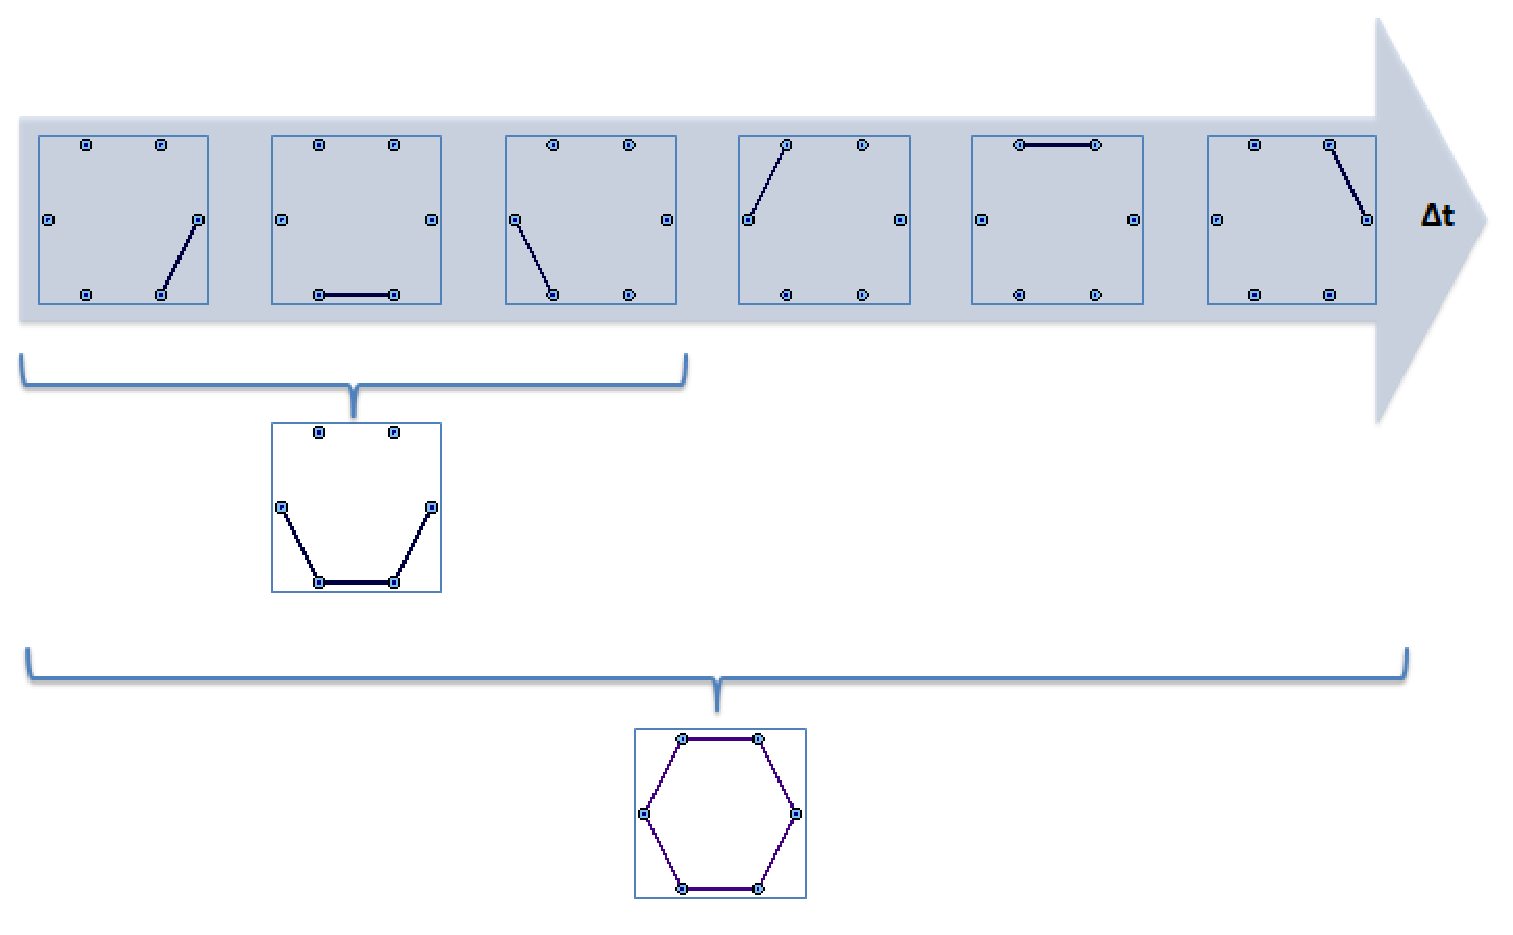
\includegraphics[width=\linewidth]{time_windows}
}

\headerbox{Einlesen eines Liedes}{name=tonformat,column=0,below=Ziel}{
Beim Start des Terminalprogramms wird eine Tabelle mit Informationen über die Tonpositionen geladen. Nach der Auswahl eines Liedes wird das Lied vom Programm eingelesen, dabei werden die Töne mit den vorher eingelesenen Tonpositionen verknüpft und die Servopositionen der Töne in einem Array gespeichert. Zusätzlich wird die Tonlänge anhand der Tempoangabe in Millisekunden umgerechnet und ebenfalls in einem Array gespeichert.
\begin{center}
	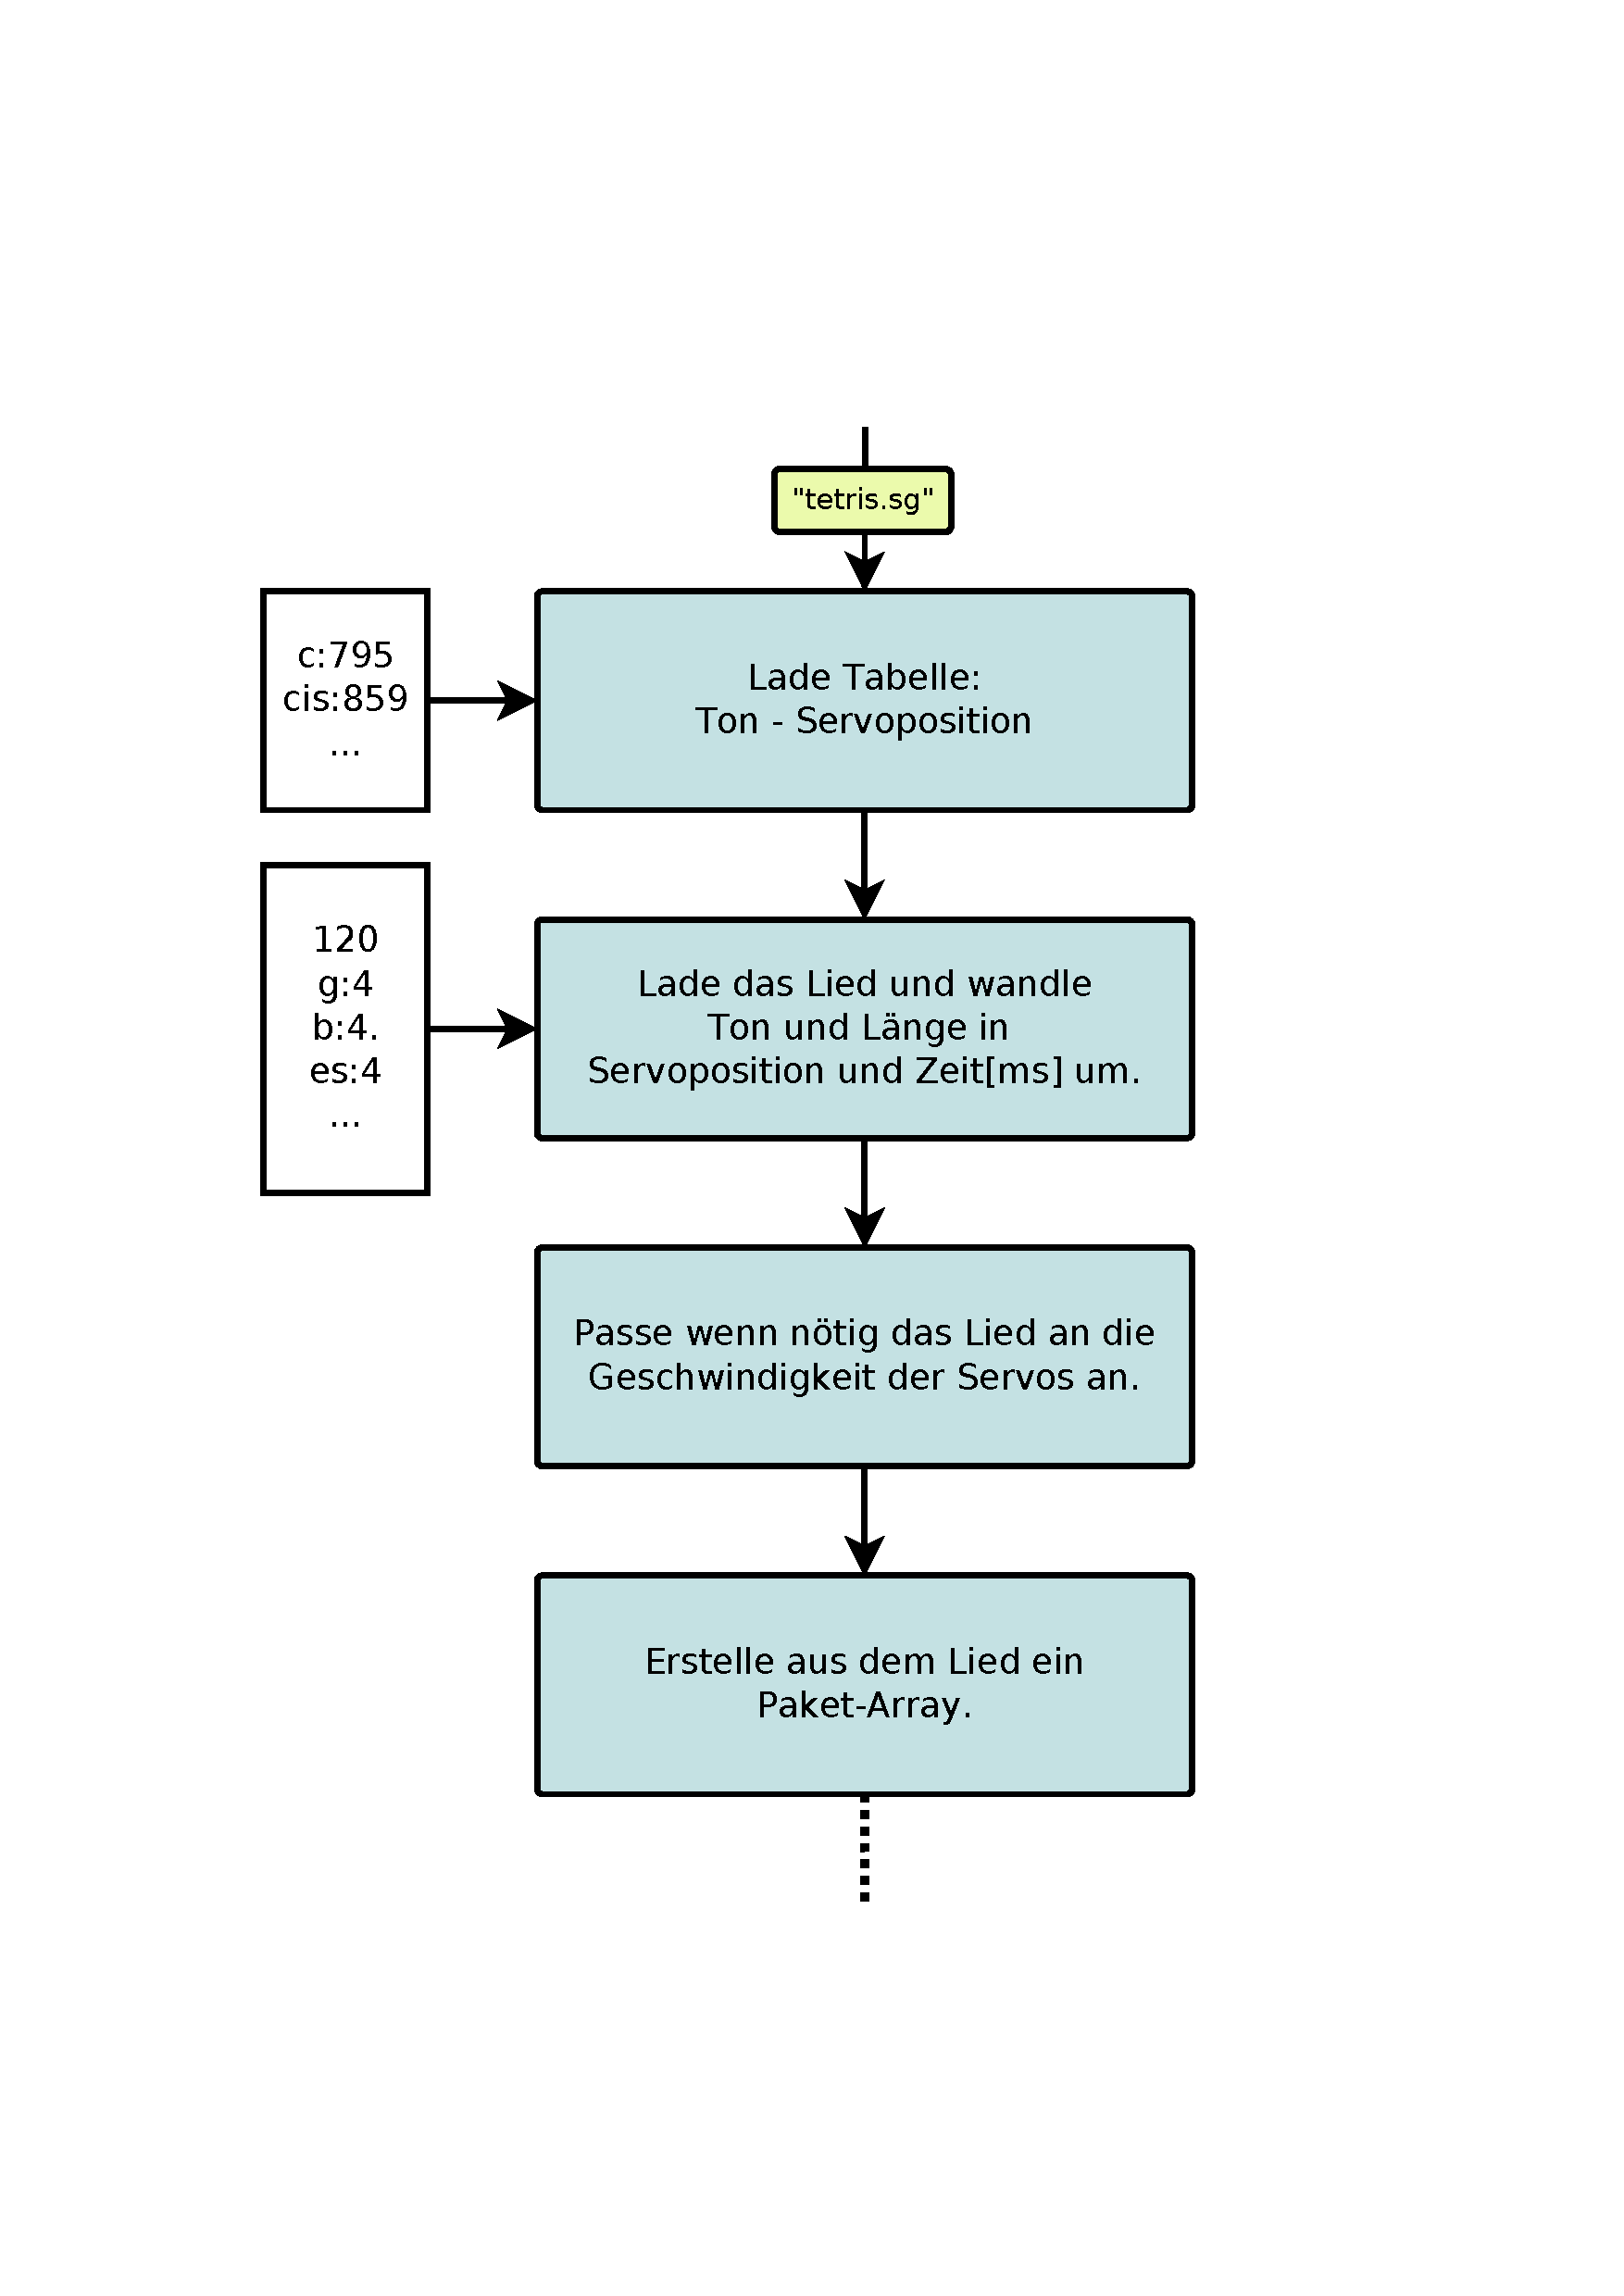
\includegraphics[trim=4.5cm 7.5cm 7.5cm 8.5cm, clip=true,height=8cm]{Bilder/Diagramm2.pdf}
\end{center}
Beim Einlesen der Töne werden Pausen direkt verarbeitet und der vorherige Ton wird um die Dauer der Pause verlängert. Diese Vereinfachung ist möglich, da bei einem Xylophon die Tonlänge konstant ist. Zum Schluss wird anhand des größten Tonabstandes, der zugehörigen Tonlänge sowie der Geschwindigkeit des Servos die maximale Liedgeschwindigkeit berechnet. Liegt diese über dem angegebenen Tempo des Liedes, so wird das Tempo des Liedes entsprechend angepasst und das Lied langsamer gespielt. Ist dies nicht der Fall, so wird das Lied in Originalgeschwindigkeit abgespielt.	
}

\headerbox{Extras}{name=references,column=0,below=tonformat,above=bottom}{
\begin{itemize}
\item grafische Benutzeroberfläche
\end{itemize}
\vspace{-0.25cm}
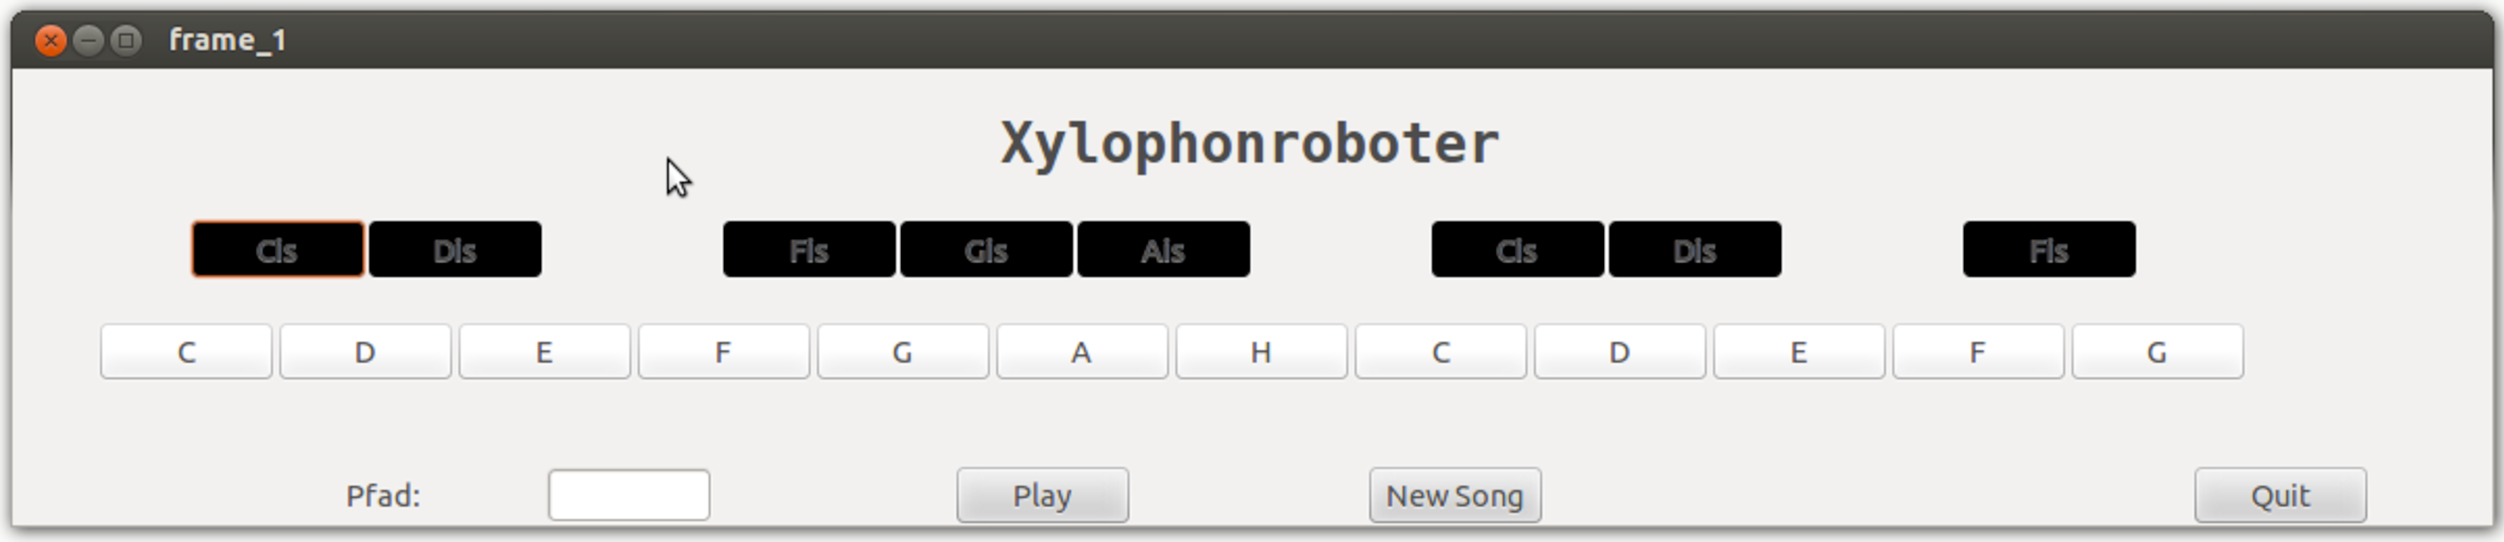
\includegraphics[width=\linewidth]{GUI}
\vspace{-0.75cm}
\begin{itemize}
\item 2 sprachige Menüführung, Übersetzung erstellt mit GNU gettext\\
http://www.gnu.org/software/gettext/
\item Tonformat kompatibel zu dem des Flötenroboters
\end{itemize}
\vspace{-0.4cm}
\footnotesize http://ornella.iwr.uni-heidelberg.de/ROBOTICSLAB/ROBPROJECTS/COMPLETED/2012PFEIFE\_A/index.html
%\vspace{1cm}
%\smaller													% Make the whole text smaller
%\vspace{-0.4em} 										% Save some space at the beginning
%\bibliographystyle{plain}							% Use plain style
%\renewcommand{\section}[2]{\vskip 0.05em}		% Omit "References" title
%\begin{thebibliography}{1}							% Simple bibliography with widest label of 1
%\itemsep=-0.01em										% Save space between the separation
%\setlength{\baselineskip}{0.4em}					% Save space with longer lines
%\bibitem{flöte} Flötenroboter Semester \emph{Projektname}, Webseite
%\end{thebibliography}
}

\headerbox{Aufbau des Xylophonroboters}{name=Aufbau,span=2,column=1,row=0}{
Der Xylophonroboter besteht aus einem halbrunden Xylophon und einem selbstgebauten Roboterarm mit zwei Servos, gesteuert durch einen Microcontroller. Alle Teile wurden auf einer Holzplatte montiert. 
\begin{center}
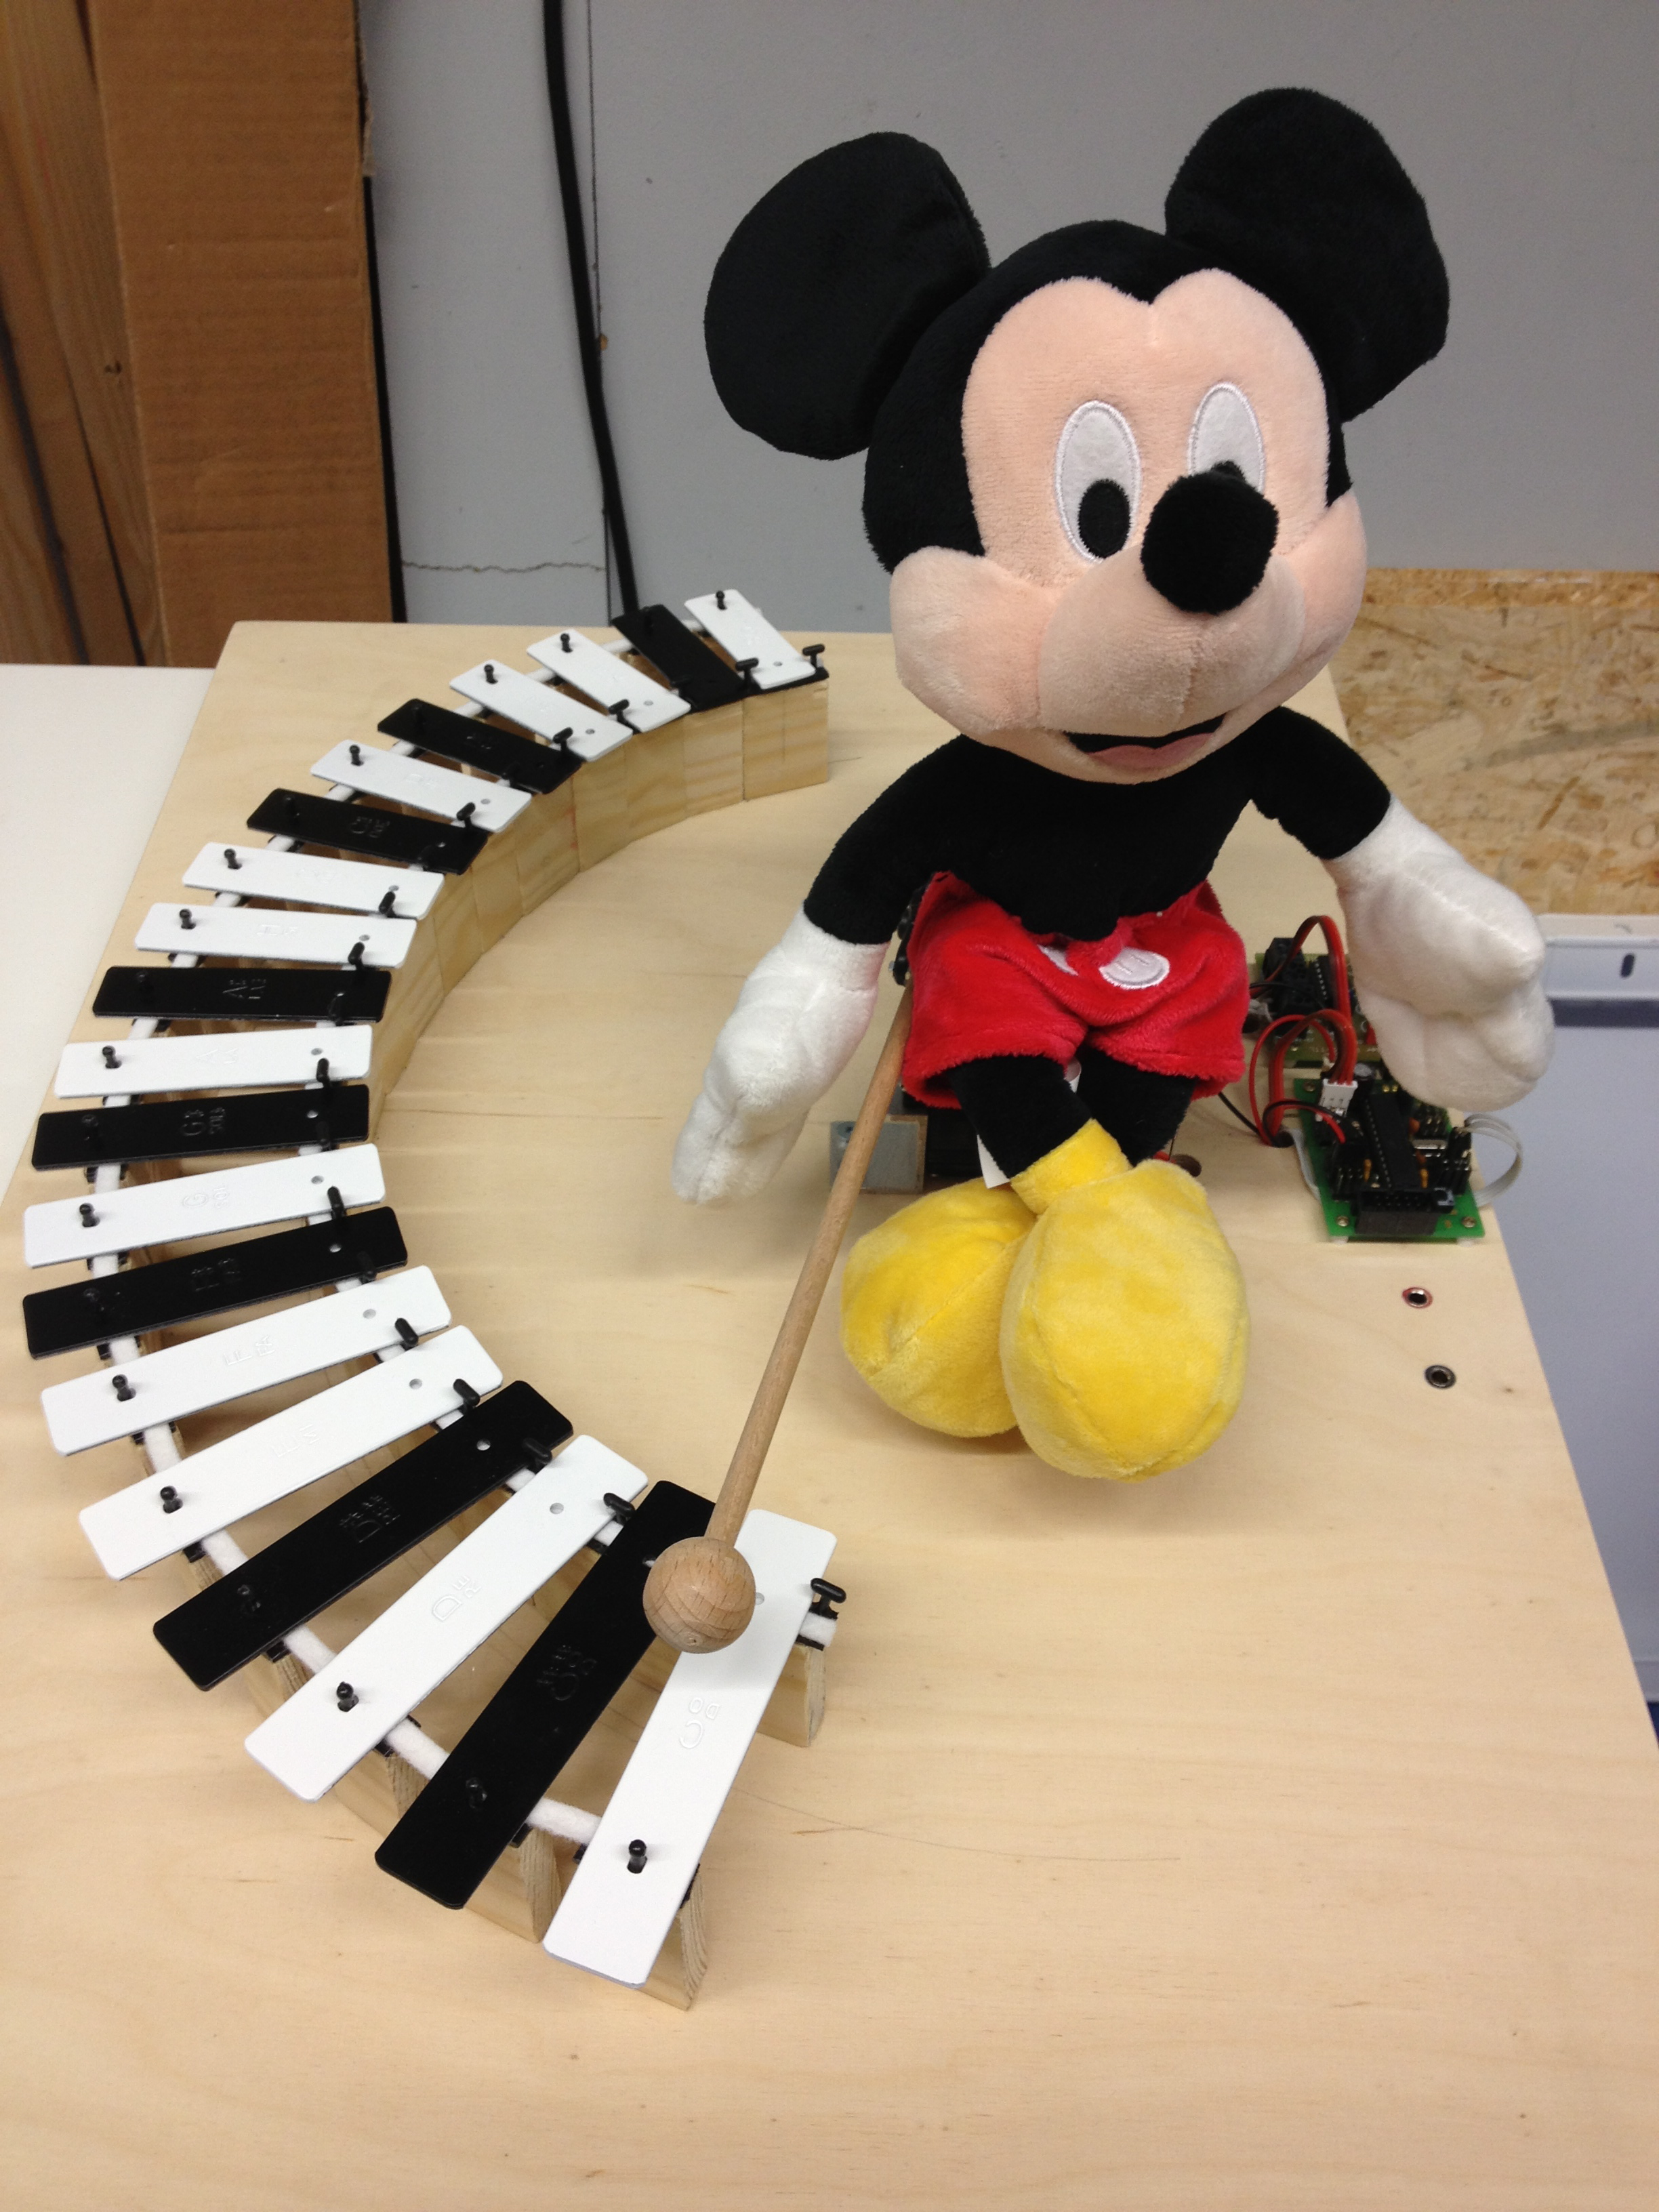
\includegraphics[trim=0cm 8cm 4cm 3cm, clip=true,width=0.34\linewidth]{Mickey.jpg}
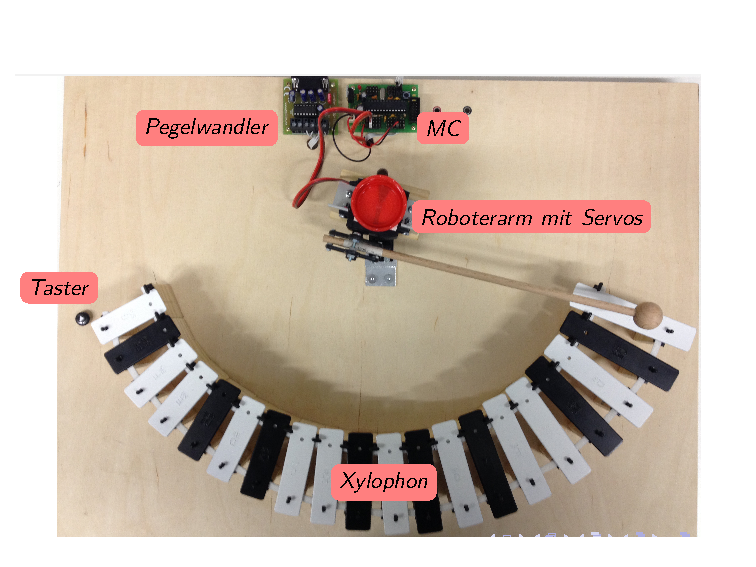
\includegraphics[trim=0cm 0.1cm 0.2cm 0.2cm, clip=true,width=0.65\linewidth]{Aufbau.pdf}
\end{center}
Ein ansprechendes Äußeres wird dem Roboter durch die abnehmbare Mickey Maus verliehen. Der Pegelwandler dient der Kommunikation mit einem PC über eine serielle Schnittstelle. Über den Taster kann der Roboter auch ohne Verbindung mit einem Computer benutzt werden. 
}

\headerbox{Steuerung}{name=konzept,span=2,column=1,below=Aufbau}{
Die Steuerung des Xylophonroboters gliedert sich in zwei Hauptbestandteile, den Mikrokontroller mit Servos und Xylophon sowie in ein Desktop-Programm, von dem aus der Roboter durch Eingabebefehle gesteuert werden kann.
Hierbei wird das Lied in einem speziellen Tonformat auf dem PC gespeichert und dann über das Terminalprogramm eingelesen, verarbeitet und dem Microcontroller paketweise per serieller Schnittstelle gesendet. Das Paket wurde ebenfalls speziell zu diesem Zweck entwickelt (siehe Desktop-Programm) und enthält die Servopositionen der Töne sowie die Tonlänge in Millisekunden. Auf dem Microcontroller befindet sich lediglich die Software, die aus den erhaltenen Paketen die Servoposition und die Tonlänge extrahiert und den entsprechenden Ton anfährt, schlägt und die Tonlänge abwartet.
}

\headerbox{Desktop-Programm}{name=desktop,span=2,column=1,below=konzept}{
\begin{multicols}{2}
%\begin{center}
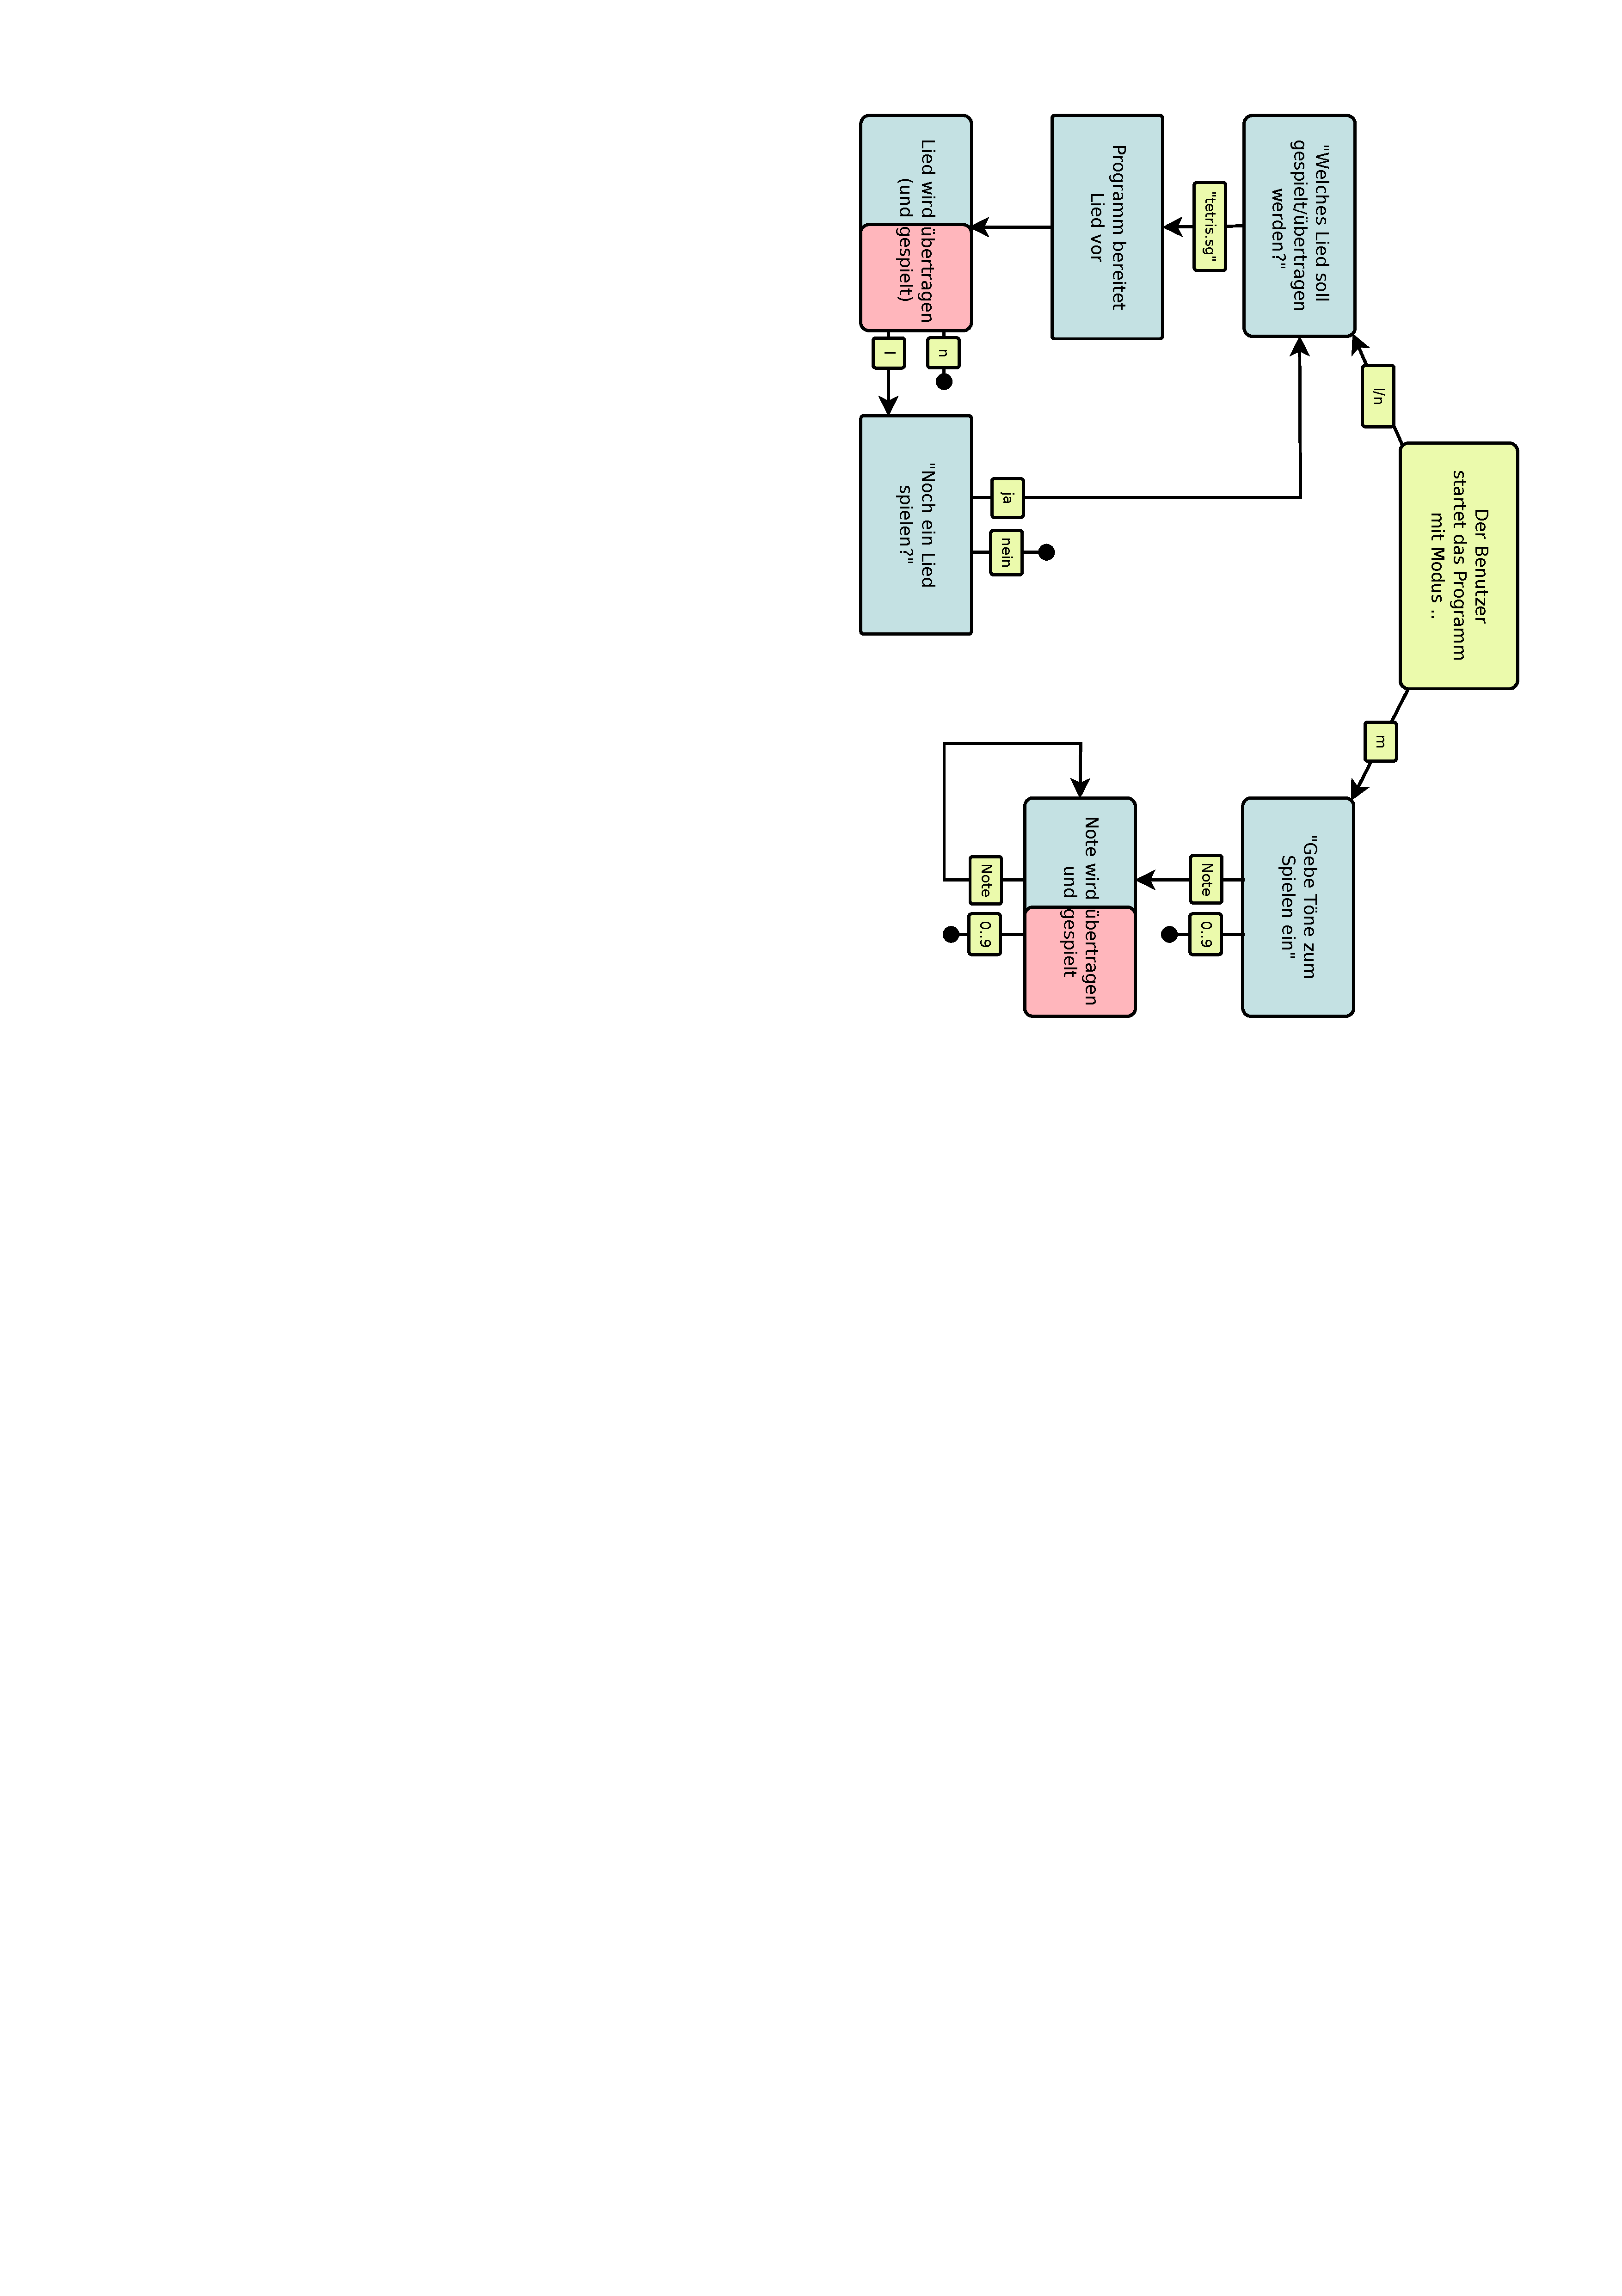
\includegraphics[trim=31.5cm 46.5cm 3.5cm 4cm, clip=true,angle=90,width=\columnwidth]{Bilder/Diagramm11.pdf}
%\end{center}
Der Roboter besitzt 3 verschiedene Betriebsmodi, die zu Beginn des Programmstarts auszuwählen sind. Man kann ihn im \textbf{"manuellen Modus"}, im \textbf{"Liedmodus"} oder zum Aufspielen eines \textbf{neuen Liedes} starten. Beim \textbf{"manuellen Modus"} können durch Eingabe der Tonnamen über die Tastatur einzelne Töne gespielt werden. Beendet wird dieser Modus durch Eingabe einer Ziffer.
Der \textbf{"Liedmodus"} und das Aufspielen eines \textbf{neuen Liedes} sind von der Menüführung fast identisch. Zu Beginn wählt man ein Lied aus einer Liste abgespeicherter Lieder oder eines selbstgeschriebenen und in dem Programmordner abgespeicherten Liedes. Beim \textbf{"Liedmodus"} wird das ausgewählte Lied direkt abgespielt, beim Aufspielen eine neuen Liedes hingegen wird das ausgewählte Lied auf dem MC gespeichert. 
\vspace{-0.5cm}
\begin{center}
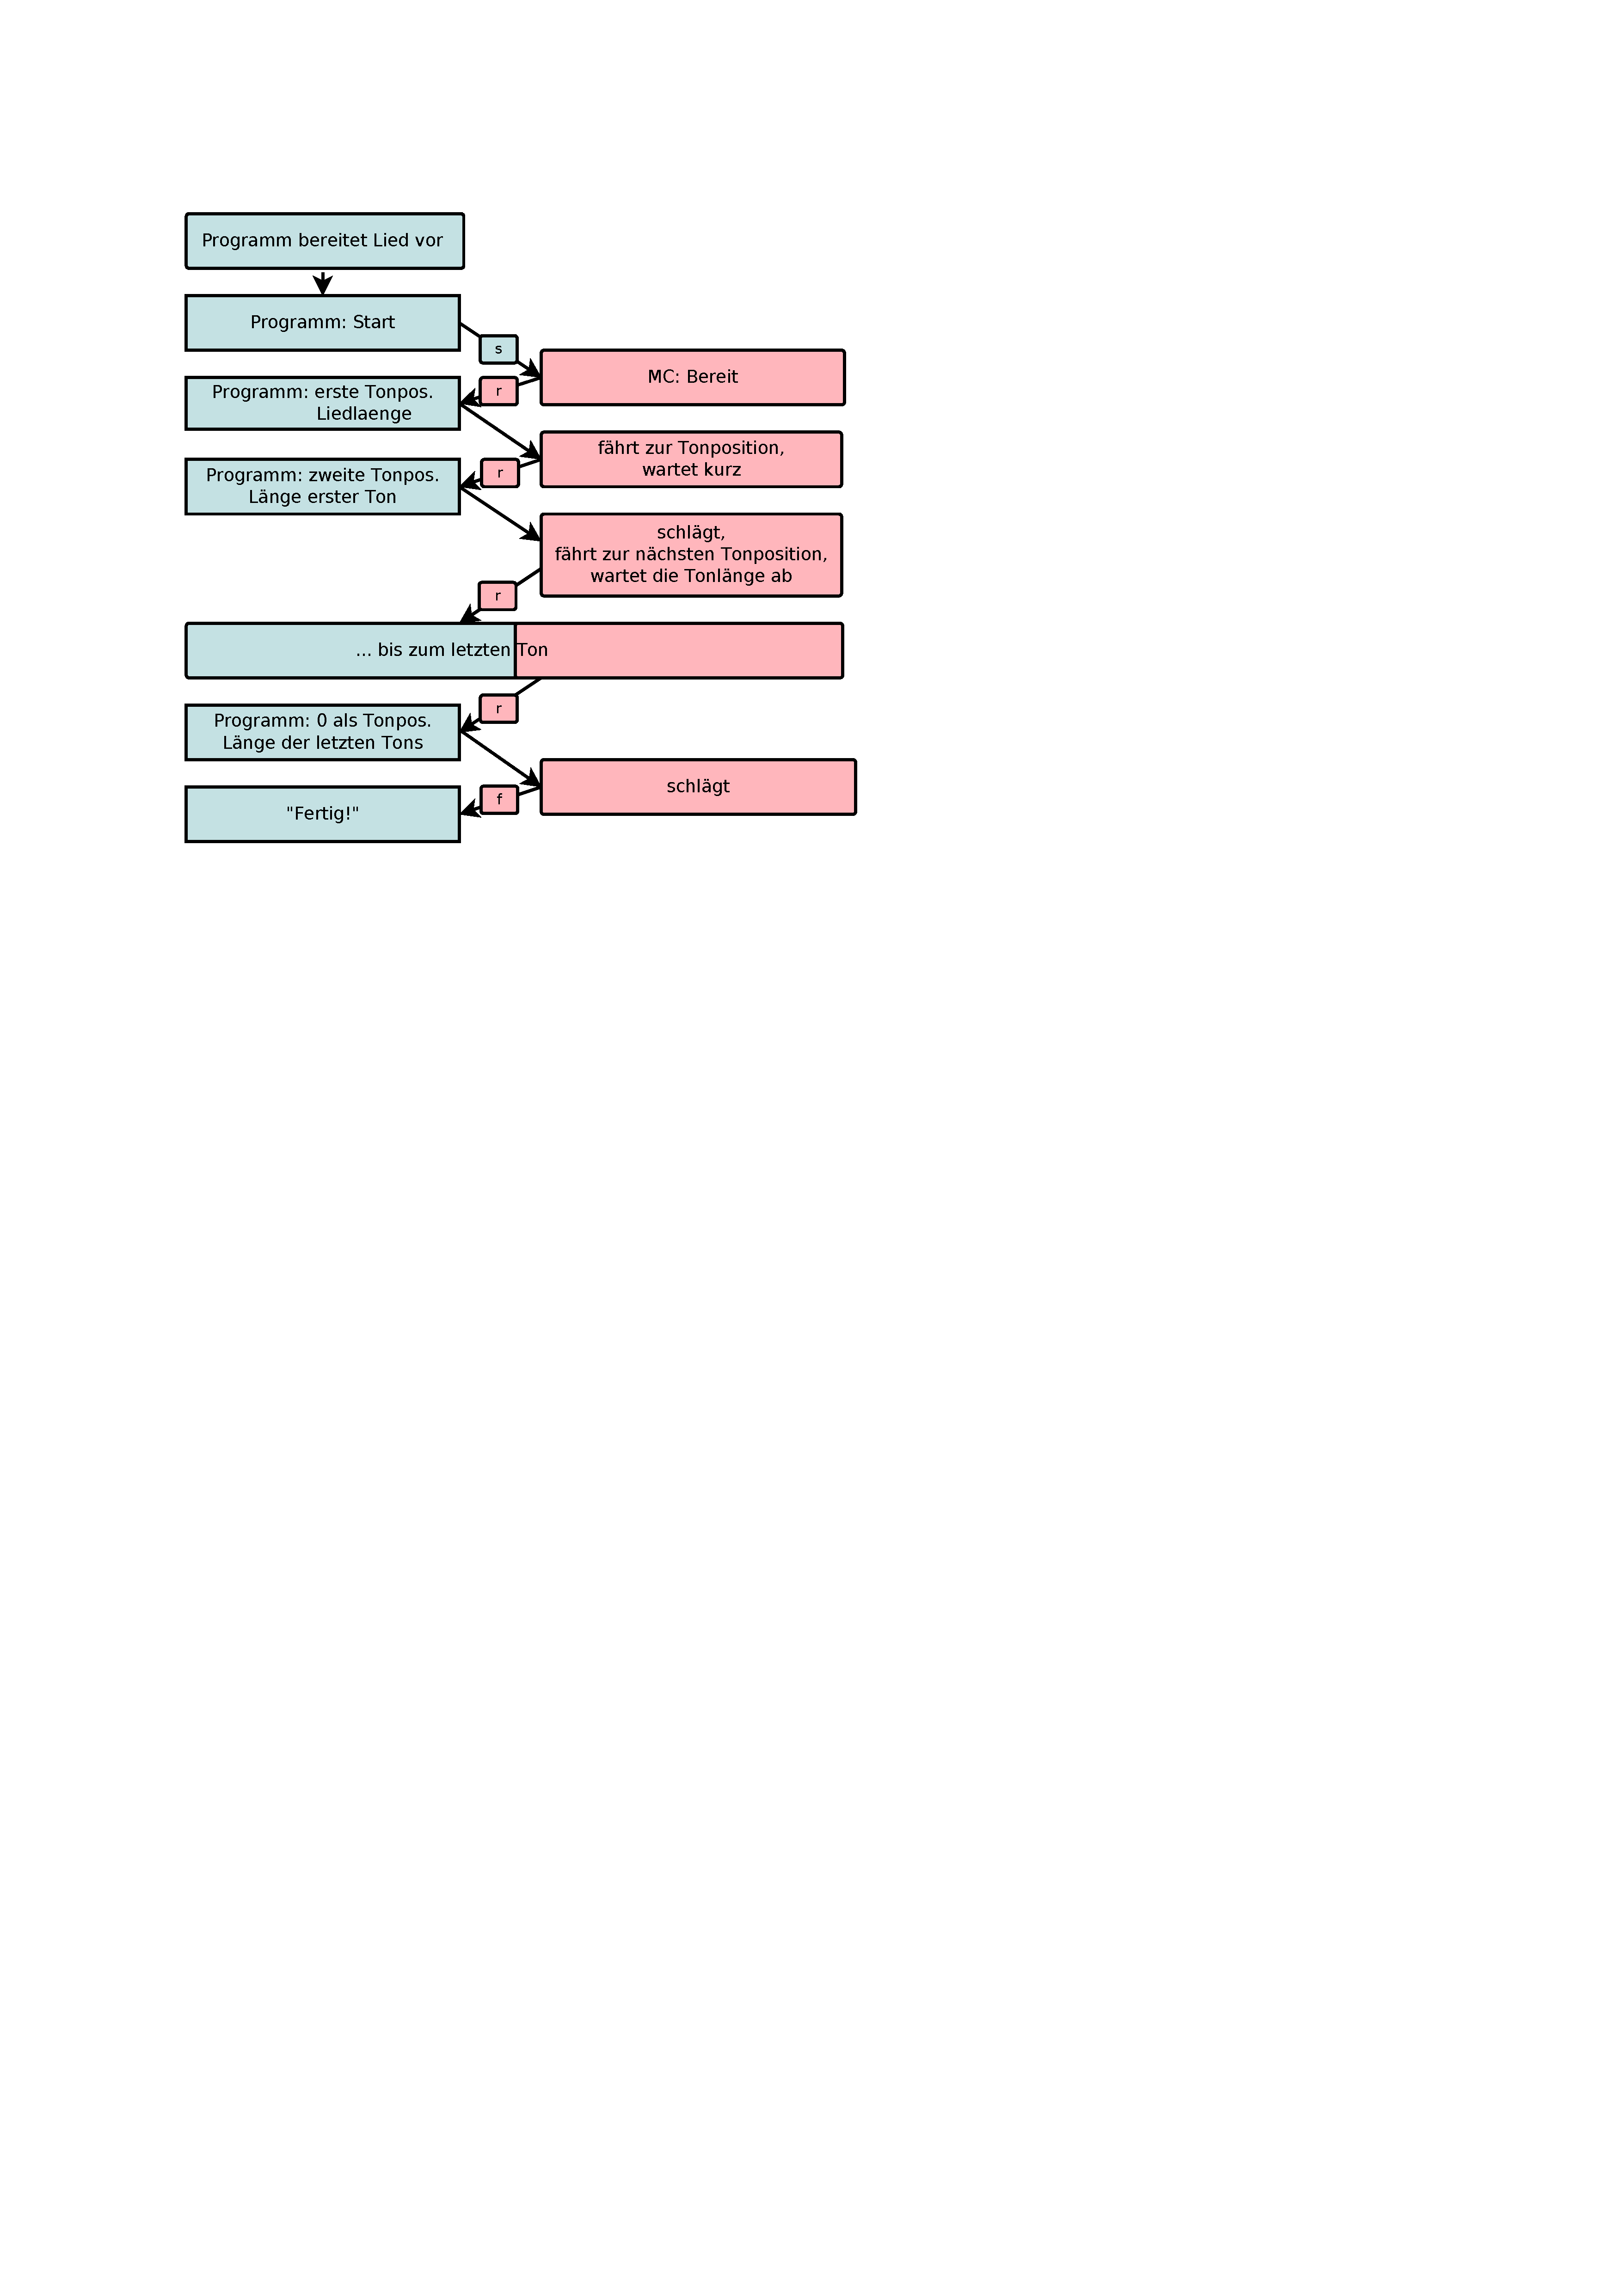
\includegraphics[trim=6.8cm 53cm 27.8cm 7.5cm, clip=true,width=6.5cm]{Bilder/Diagramm3.pdf}
\end{center}
\end{multicols}
}

\headerbox{Weiterentwicklung}{name=ausblick,column=1,below=desktop,above=bottom}{
%Zur Weiterentwicklung bzw. Verbesserung des Roboters können folgende Punkte umgesetzt werden:
\begin{itemize}
%\vspace{-0.2cm}
	\item Synchronisation/Zusammenspiel mit anderen Instrumentalrobotern, z.B. Flötenroboter
%\vspace{-0.65cm}
	\item Einbinden von MIDI Datein
%\vspace{-0.2cm}
	\item Modifizieren des manuellen Modus
%\vspace{-0.2cm}
	\item Verbesserung der grafischen Benutzeroberfläche
\end{itemize}
%\includegraphics[angle=-90,width=0.49\linewidth]{team.jpg}
} 

\headerbox{Das Team}{name=team,column=2,below=desktop,above=bottom}{
%\smaller						% Make the whole text smaller
%\vspace{-0.4em}			% Save some space at the beginning
\center
Simon Stemmle\\
5. Semester Physik\\
Stemmle@stud.uni-heidelberg.de\\
\vspace{0.3cm}
Tobias Buck\\
5. Semester Physik\\
buck@stud.uni-heidelberg.de\\
%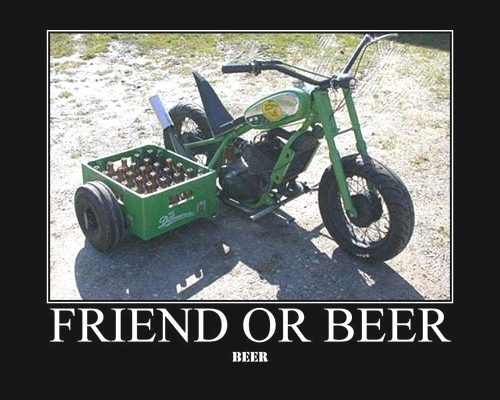
\includegraphics[width=1\linewidth]{23uhr.jpg}
} 

\end{poster}
\end{document}
